\renewcommand{\thefootnote}{\fnsymbol{footnote}}

\chapter[Stochastic dominance and applications]%
 {Stochastic dominance and applications}%
\label{ch:L4}

% 3) Reset things so later footnotes go back to 1, 2, 3, …
%\setcounter{footnote}{0}
\renewcommand{\thefootnote}{\arabic{footnote}}

\section{Stochastic dominance}\label{sec:L4-intro}

In Lecture \ref{ch:L3}, we developed an analysis of properties of expected utility preferences. However, we have not yet discussed relevant properties of lotteries, which is what we do now.

To start, one might want to have a language to say that a \textquote{lottery yields higher returns than another one}. A simple way of capturing this idea is the following: an individual with expected utility preferences should prefer lottery \( F \) to lottery \( G \) for any possibile utility function \( u \). This is first-order stochastic dominance.

\begin{definition}\label{def:fosd}
	The lottery \( F \) \textbf{first-order stochastically dominates} \( G \) if
	\begin{equation}\label{eq:fosd1}
		\int u(x) dF(x) \geq \int u(x) d G(x) \quad \text{for every nondecreasing } u.
	\end{equation}
\end{definition}


There is a second way of capturing the idea: for each given return, the probability of getting at least that return is higher in one lottery than in the other one. That is, for each return \( x \), if \( F(x) \leq G(x) \), then the probability of getting at least \( x \) is higher in lottery \( F \) than in lottery \( G \), because the probability of getting at least \( x \) in lottery \( F \) is \( 1-F(x) \). The two criteria \eqref{def:fosd} and \( F(x) \leq G(x) \) are equivalent, as stated by the following result.

\begin{proposition}\label{prop:fosd}
	Lottery \( F \) first-order stochastically dominates lottery \( G \) if and only if \( F(x) \leq G(x) \).
\end{proposition}

You are asked to prove one direction of Proposition \ref{prop:fosd} in Exercise \ref{ex:fosd-ex}. As illustrated in Figure \ref{fig:fosd}, lottery \( F \) first-order stochastically dominates lottery \( G \) if its graph is always below the graph of lottery \( G \).

\begin{figure}[H]
	\centering
	\tikzset{every picture/.style={line width=0.75pt}} %set default line width to 0.75pt        

	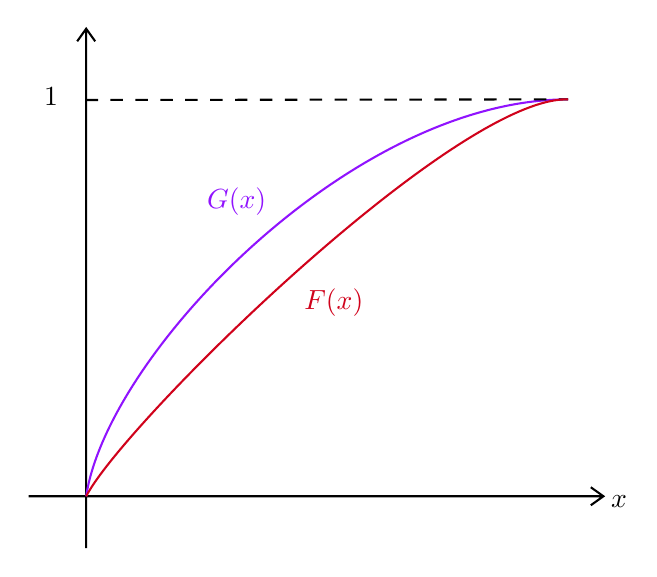
\begin{tikzpicture}[x=0.65pt,y=0.65pt,yscale=-1,xscale=1]
		%uncomment if require: \path (0,349); %set diagram left start at 0, and has height of 349

		%Shape: Axis 2D [id:dp8000510474681485] 
		\draw  (160,302.32) -- (479.48,302.32)(191.95,42.4) -- (191.95,331.2) (472.48,297.32) -- (479.48,302.32) -- (472.48,307.32) (186.95,49.4) -- (191.95,42.4) -- (196.95,49.4)  ;
		%Curve Lines [id:da5171104107126938] 
		\draw [color={rgb, 255:red, 144; green, 19; blue, 254 }  ,draw opacity=1 ]   (191.95,302.32) .. controls (203.57,223.81) and (339.39,81.68) .. (459.83,81.68) ;
		%Straight Lines [id:da9399220418666737] 
		\draw  [dash pattern={on 4.5pt off 4.5pt}]  (191.61,82.02) -- (459.83,81.68) ;
		%Curve Lines [id:da8164662036086425] 
		\draw [color={rgb, 255:red, 208; green, 2; blue, 27 }  ,draw opacity=1 ]   (191.95,302.32) .. controls (212.96,261.57) and (397.47,80) .. (459.83,81.68) ;

		% Text Node
		\draw (482.02,300.33) node [anchor=north west][inner sep=0.75pt]    {$x$};
		% Text Node
		\draw (166.81,73.24) node [anchor=north west][inner sep=0.75pt]    {$1$};
		% Text Node
		\draw (311.5,185.35) node [anchor=north west][inner sep=0.75pt]  [color={rgb, 255:red, 208; green, 2; blue, 27 }  ,opacity=1 ]  {$F( x)$};
		% Text Node
		\draw (257.47,128.87) node [anchor=north west][inner sep=0.75pt]  [color={rgb, 255:red, 144; green, 19; blue, 254 }  ,opacity=1 ]  {$G( x)$};


	\end{tikzpicture}
	\caption{Lottery \( F \) first-order stochastically dominates lottery \( G \).}
	\label{fig:fosd}
\end{figure}

Notice that first-order stochastic dominance is an \textit{incomplete} ordering over lotteries: there are pairs of lotteries \( F, G \) such that neither \( F \) first-order stochastically dominates \( G \) nor \( G \) first-order stochastically dominates \( F \).

First order stochastic dominance is a comparison of returns. We now develop a notion allowing us to compare riskiness. Again, we start from an intuitive idea: say that two lotteries have the same expected return, but a risk averter prefers one lottery to the other. Since the individual is risk averse, she must be preferring the less risky lottery. In this case, we say that the first lottery second-order stochastically dominates the second one.

\begin{definition}\label{def:sosd}
	The lottery \( F \) \textbf{second-order stochastically dominates} \( G \) with the same mean if

	\[
		\int u(x) d F(x) \geq \int u(x) dG(x) \quad \text{for every nondecreasing concave } u.
	\]
\end{definition}

Recall that if an expected utility maximiser has a concave utility function, he is risk averse, which explains the qualifier in Definition \ref{def:sosd}.

There is a second intuitive way of defining second-order stochastic dominance using the concept of a \textit{mean preserving spread}. Consider the following compound lottery. First, an outcome \( x \) is drawn according to a distribution \( F \). Then, to the realisation \( x \), an amount \( z \), distributed according to a distribution with mean zero, is added. The resulting lottery has the same mean as \( F \) but is more spread out, hence riskier. Such a lottery is called a mean preserving spread of \( F \). If a lottery \( G \) can be constructed in this way from lottery \( F \), we say that \( G \) is a mean preserving spread of \( F \). We have the following result.

\begin{proposition}\label{prop:sosd}
	If two distributions \( F \) have the same mean \( G \), then \( F \) second-order stochastically dominates \( G \) if and only if \( G \) is a mean preserving spread of \( F \).
\end{proposition}

\section{Applications}

We conclude our treatment of (objective) expected utility theory with two applications of the concepts developed so far: insurance and investment in a risky asset.

\paragraph{Insurance.} Consider an expected utility maximiser with initial wealth \( w>0 \) who faces a possible loss \( D>0 \). The loss occurs with probability \( \pi \in (0,1) \) and does not occur with probability \( 1-\pi \). It is possible to buy insurance: one unit of insurance costs \( q \) euros for sure and pays \( 1 \) euro if the loss occurs.

If the individual buys \( \alpha \ge 0 \) units of insurance, his decision problem is

\begin{equation}\label{eq:insurance-problem}
	\max_{\alpha \ge 0} \Big\{ (1-\pi)\,u(w-\alpha q)
	+ \pi\,u(w - D - \alpha q + \alpha) \Big\}.
\end{equation}

Assume an interior optimum \( \alpha^*>0 \). Differentiating Equation \eqref{eq:insurance-problem} with respect to \( \alpha \) gives
\[
	(1-\pi)\,u'(w-\alpha q)(-q)
	+ \pi\,u'(w - D - \alpha q + \alpha)\,(1-q),
\]

so \( \alpha^* \) satisfies

\[
	(1-\pi)\,u'(w-\alpha^* q)(-q)
	+ \pi\,u'(w - D - \alpha^* q + \alpha^*)\,(1-q) = 0.
\]

If the individual is risk neutral, and therefore \( u \) is linear, the individual maximises expected wealth:

\[
	w - \pi D + \alpha(\pi - q) .
\]

The solution depends on the relationship between the insurance price \( q \) and the probability \( \pi \):

\begin{itemize}
	\item If \( \pi = q \), then \( \pi - q = 0 \) and expected wealth

	      \[
		      w - \pi D
	      \]

	      is constant in \( \alpha \). Expected wealth is the same for every \( \alpha \), so the decision maker is indifferent over all insurance levels.

	\item If \( \pi < q \), then the slope \( \pi - q < 0 \), so expected wealth
	      \[
		      w - \pi D + \alpha(\pi - q)
	      \]
	      is strictly decreasing in \( \alpha \). Expected wealth is maximised by choosing no insurance, \( \alpha^* = 0 \).
\end{itemize}

If the individual is risk averse, and therefore \( u \) is strictly concave, then:

\begin{itemize}
	\item With \emph{fair insurance}, \( q=\pi \), expected wealth does not depend on \( \alpha \), but full insurance, \( \alpha = D \), makes wealth non-random, as it is \( w - \pi D \) in both states. A strictly risk-averse individual strictly prefers this certainty and chooses full insurance. You are asked to verify this claim in Exercise \ref{ex:insurance-full}.
	\item With \emph{loaded insurance}, \( q>\pi \), expected wealth decreases in \( \alpha \), but insurance reduces risk. A strictly risk-averse decision maker may still choose a strictly positive but finite \( \alpha^* \), characterised by the first-order condition above.
\end{itemize}

\paragraph{Risky asset} Consider an investor with expected utility preferences and initial wealth \( w>0 \). There are two assets: a \emph{safe asset} with sure return \( 1 \) per euro invested; a \emph{risky asset} with random return \( z \) per euro invested, with distribution \( F \) and

\begin{equation}\label{eq:risky-asset-mean}
	\int z \, dF(z) > 1,
\end{equation}

so that the risky asset has higher expected return than the safe asset.

Let \( \alpha \) denote the amount invested in the risky asset and \( \beta \) the amount invested in the safe asset. The budget constraint is

\[
	\alpha + \beta = w, \qquad \alpha,\beta \ge 0.
\]

For any realization \(z\), final wealth is

\[
	\alpha z + \beta.
\]

Using the budget constraint \(\beta = w - \alpha\), we can rewrite wealth as

\[
	\alpha z + (w - \alpha) = w + \alpha(z-1).
\]

We now use the expectation notation \( \mathbb{E} \), omitting the CDF \( F \) for simplicity. The investor's problem is thus

\begin{equation}\label{eq:risky-asset-problem}
	\max_{0 \le \alpha \le w} \; \mathbb{E}\big[ u\big( w + \alpha (z-1) \big) \big].
\end{equation}

Suppose the optimum is interior, \( \alpha^* \in (0,w) \). Then the first-order condition for \( \alpha^* \) is

\[
	\mathbb{E}\big[\,u'\big(w + \alpha^*(z-1)\big)\,(z-1)\,\big] = 0.
\]

Notice that this condition resembles the one we obtained for insurance. In each case, the individual trades off marginal utility in different states weighted by the \textquote{per-unit payoff difference} in that state.

If the individual is risk neutral and therefore \(u\) is linear, then \(u'\) is constant and the condition reduces to

\[
	\mathbb{E}[z-1] = 0.
\]

Since \( \mathbb{E}[z] > 1 \) by Equation \eqref{eq:risky-asset-mean}, \( \mathbb{E}[z-1] > 0 \), so the derivative of expected utility is positive for all \( \alpha \) and the optimum is a corner: \( \alpha^* = w \), all wealth is invested in the risky asset.

If instead \( u \) is strictly concave, then \( u' \) is decreasing, so high-\( z \) states, where wealth is high, are given less weight and low-\( z \) states are given more weight. The higher expected return of the risky asset is traded off against the disutility of risk, and this typically yields an interior solution \( 0 < \alpha^* < w \).

If \( u \) is twice differentiable and strictly concave, then the second derivative of expected utility with respect to \( \alpha \) is

\[
	\mathbb{E}\big[\,u''\big(w + \alpha(z-1)\big)\,(z-1)^2\,\big] < 0,
\]

since  \( (z-1)^2 \geq 0 \) and \( u''<0 \). Hence expected utility is strictly concave in \( \alpha \), so any solution to the first-order condition is the unique global maximizer.

Evaluating the derivative at \( \alpha = 0 \) gives

\[
	\mathbb{E}\big[\,u'(w)(z-1)\big]
	= u'(w)\,\mathbb{E}[z-1].
\]

If \( \mathbb{E}[z]>1 \), then \( \mathbb{E}[z-1]>0 \), so the derivative at \( \alpha=0 \) is positive and the individual strictly prefers to hold a positive amount of the risky asset.

From the condition

\[
	\mathbb{E}\big[\,u'\big(w + \alpha^*(z-1)\big)\,(z-1)\,\big] = 0,
\]

one could argue that the optimal risky position \( \alpha^* \) decreases if the individual becomes more risk averse. That is, \( u \) becomes more concave, so bad states are weighted more heavily through \( u' \). The moral of the story is: if a risk is actuarially favourable, a risk-averse individual will invest in it, but the more risk averse she is, the less she will invest.

\paragraph{Things to read.} Most of this lecture draws from \citet[ch. 6.D.]{mas-colellMicroeconomicTheory1995}, you can find an alternative treatment in \citet{krepsMicroeconomicFoundations2013}.

\section{Exercises}

\begin{exercise}\label{ex:fosd-ex}
	Prove one direction of Proposition \ref{prop:fosd}: show that if \( F \) first-order stochastically dominates \( G \) in the sense of Definition \ref{def:fosd}, then \( F(x) \leq G(x) \). (check \citet[p. 195]{mas-colellMicroeconomicTheory1995} if you are stuck)
\end{exercise}

\begin{exercise}
	There is another way of defining first-order stochastic dominance. Consider the following compound lottery. First, an outcome \( x \) is drawn according to a distribution \( F \). Then, to the realisation \( x\), an amount \( z \), distributed according to \( G \), is added. Show that such a compound lottery first-order stochastically dominates \( F \). The reserve also hold: if \( F \) first-order stochastically dominates \( G \), then \( F \) can be constructed as a compound lottery as above!
\end{exercise}

\begin{exercise}
	Prove one direction of Proposition \ref{prop:sosd}, if \( G \) is a mean preserving spread of \( F \), then \( F \) second-order stochastically dominates \( G \). (check \citet[p. 197]{mas-colellMicroeconomicTheory1995} if you are stuck)
\end{exercise}

\begin{exercise}\label{ex:insurance-full}
	Consider the insurance problem in Equation \eqref{eq:insurance-problem} with fair insurance, \( q=\pi \). Show that full insurance, \( \alpha = D \), is optimal for a risk-averse individual.
\end{exercise}

\bibliographystyle{apacite}  % or another  style
\bibliography{references} % .bib file goes in ./bib/